\documentclass[review]{elsarticle}

\usepackage[final]{pdfpages}
\usepackage[margin=1in]{geometry}
\usepackage{lineno,hyperref,subfig, graphicx,epstopdf}
\modulolinenumbers[5]

\journal{Journal of XXX}

\bibliographystyle{elsarticle-num}

\begin{document}

\begin{frontmatter}

\title{Flood Water Segmentation for Crowdsourced Images}

\author[mymainaddress]{John K. Nguyen\corref{mycorrespondingauthor}}
\address[mymainaddress]{Illinois Informatics Institute, University of Illinois at Urbana-Champaign}

\author[mysecondaryaddress]{Barbara S. Minsker}
\cortext[mycorrespondingauthor]{Corresponding author}

\address[mysecondaryaddress]{Civil \& Environmental Engineering Department, Southern Methodist University}

\begin{abstract}
The proliferation of camera-equiped mobile devices have led to a new source of information for flood research. In-situ photographs captured by people provides information at the local level that remotely sensed images fail to capture. Applications of crowdsourced images to flood research requires understanding the content of the image without the need for user-input. This paper addresses the problem of how to automatically determine a flooded and non-flood region in crowdsourced images. Previous works required two images taken at similar angle and perspective of the location when it is flooded and when it is not flooded. We examine three different algorithms that is able to perform segmentation using a single flood image without these assumptions. The performance of each algorithm is evaluated on a collection of crowdsourced flood images. We show that it is possible to accurately segment a flood image using just a single image.
\end{abstract}

\begin{keyword}
flood water segmentation \sep crowdsourcing \sep image processing \sep computer vision
\end{keyword}

\end{frontmatter}

\linenumbers

\section{Introduction}

The use of crowdsourced information in floods is a very recent active research area. In \cite{poser}, the quality of geographic information gathered from an flood-affected population was compared to hydraulic models. The authors found that the affected population was able to estimate flood water level as accurate as hydraulic models. Another study on the quality of crowdsourced information for flood research was given by \cite{moreira}. In a case study on flood risk assessment for Sao Carlos, Brazil watershed, the authors found that the volunteered geographic information is comparable to data collected from sensors. The usefulness of crowdsourced geographic information have led to the development of cyber-infrastructure systems and decision-support tools with crowdsourcing capabilities \cite{wan, lieske, horita}. These tools allow the public and emergency responders to input information such as severity classification, number of fatalities, and flood duration.

As more and more people become equipped with mobile phones with camera capability, photographs and videos are becoming a very common medium of information.  Crowdsourced photographs pose new opportunities for flood research which have traditionally relied on remotely sensed radar and satellite images for flood risk assessment \cite{youssef, robertson}, flood mapping \cite{hanhmann}, flood monitoring \cite{tholey, khan}, and flood damage assessment \cite{tralli, sande}. While remotely sensed images provides wholistic analysis of an entire region, they do not capture information at the local level. For example, information such as flood depth is more accurate from an in-situ image than depth sensors located far from the inundated area \cite{ko}.

The first major usage of crowdsourced flood images for flood research is the FP7 SPACE Project GEO-PICTURES, a collaborative effort between the United Nations (UNOSAT) and AnsuR Technologies \cite{unosat}. Through a mobile-app called UN-ASIGN, crowdsourced, geo-tagged photos captured on smartphones were used in conjunction with radar images to improve flood assessment. Using the data collected from the 2011 Thailand floods, the Thai government and Asian Disaster Prevention Center developed better emergency management response.

As crowdsourced flood images become incorporated into future decision-support tools, there is a need to automatically process images. One of the fundamental problems in working with crowdsourced flood images is  \emph{flood water segmentation}, the partition of the flooded region from the rest of the image. To automate such a task poses a major challenge due to the lack of standardization, quality assurance, or quality control. Consider remotely sensed LiDAR images which must follow the base specifications for quality dictated by U.S. Geological Survey (USGS) \cite{heidemann}. Standardized images such as LiDAR makes the application of image processing much easier as there is limited variability in how the image was captured and its content. Crowdsourced images, however, could be taken from different elevations with varying angles, be of extremely poor or high quality, and may contain numerous visible objects (e.g., people, trees, cars, etc.). Algorithms to segment the flood water from crowdsourced images must be able to work with the gamut of information contained in each image.

\section{Related Work \& Contributions}

There have been several previous work in segmenting flood water from images for the purpose of water level detection. The common assumption of these works is that all images taken are at a consistent perspective and angle from a pre-calibrated camera. The paper by \cite{park} utilize the accumulated histogram which shows changes in a sequence of images. To separate the water and non-water region, the authors used a bandpass filter is used to remove noise and a set of decision rules based on the pulse histograms of each image. Another image differencing approach was used in \cite{yu} to detect changes in water level. Using a reference image and a acquisition image from a pre-calibrated camera, the change between the two images was determined by comparing the change in the Y-axis profile of the Sobel edge image. We direct the readers to \cite{ko} for a comprehensive survey of other image differencing approaches to this problem.

The use of crowdsourced flood images for water level detection was introduced in \cite{narayanan}. Participants captured and upload a geo-tagged image of a flood containing submerged static structures such as a building and lampposts. Then, using a previously stored reference image, a flood line is estimated based on invariant feature transform (SIFT). The segmentation of flood and non-flood regions in crowdsourced flood images was studied more generally in \cite{witherow}. Using a non-flood and a flood image of the same location, the authors determine the flood region via image subtraction based on the specularity (i.e., reflection) of the flood water between the two images.

Many of the works in water level detection presented above is not applicable for all flood images as they assume pre-calibrated cameras. Also, within the context of crowdsourcing, it is not possible to apply image differencing approaches in general as a non-flood image of the exact location might not be available or might not have been taken with the same conditions as the flood image. In this work, we relax the assumption of a pre-calibrated camera and the need for two images.

The main contribution of this paper is to show that we can perform flood water segmentation from just a single  crowdsourced image. We make no assumptions on how the image was captured and its content. We propose three algorithms used in the image processing and computer vision to this problem. The performance of the algorithms is evaluated on a real dataset of crowdsource images taken from different flood events. Discussions on how to improve the performance of both algorithms as well as future research using crowdsourced flood images will be also given.

\section{Crowdsourced Flood Image Dataset}

The dataset used in this paper consists of 25 publicly available in-situ flood images taken from different flooding events. To simulate real-world application, these images are of different dimensions, taken with different perspectives and angle, and contain high variability in content. Some characterization of the images includes:

\begin{itemize}
\item {\bf Slanted or non-linear water horizon}: All images either contains a slanted water horizon or a non-linear horizon.
\item {\bf Ambiguous water horizon}: The water horizon in a flood image may be ambiguous or there can be multiple horizons.
\item {\bf Lack of color features}: As floods occur during or after a storm, the color information of the image might be limited, making it difficult to classify if a pixel belongs to the water region or the sky region.
\item {\bf Present of objects}: There might exist objects on the water horizon such as cars, people, and debris.
\end{itemize}
Most of the images in our dataset will contain a combination of these characterizations. A sample of the images used is provided in Figure \ref{fig:example}.

\begin{figure}
\begin{tabular}{ccc}
\subfloat[]{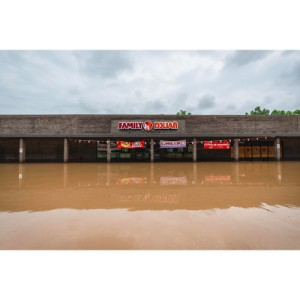
\includegraphics[width = 2in]{images/example_image1.jpg}} &
\subfloat[]{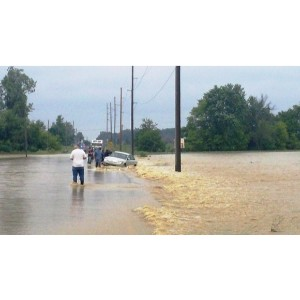
\includegraphics[width = 2in]{images/example_image2.jpg}} &
\subfloat[]{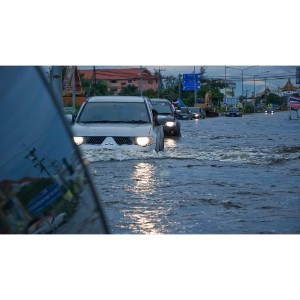
\includegraphics[width = 2in]{images/example_image3.jpg}} \\
\subfloat[]{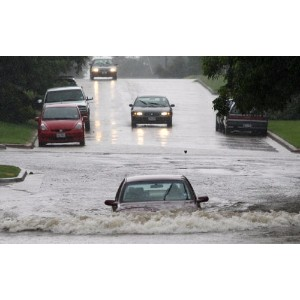
\includegraphics[width = 2in]{images/example_image4.jpg}} &
\subfloat[]{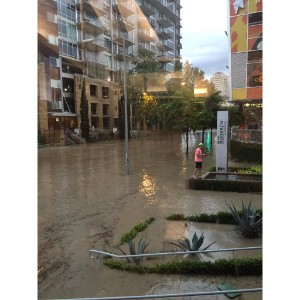
\includegraphics[width = 2in]{images/example_image5.jpg}} &
\subfloat[]{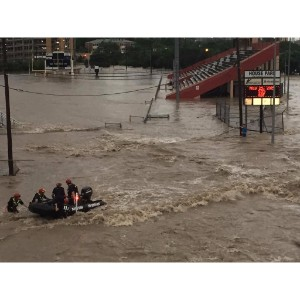
\includegraphics[width = 2in]{images/example_image6.jpg}} 
\end{tabular}
\caption{Examples of images contained in the dataset.}
\label{fig:example}
\end{figure}

\section{Methodologies}\label{sec:water_seg}

We present two algorithms which are applicable for the flood water segmentation problem. The first algorithm is found in the domain of image processing where we segment an image based on transformations and local operations at the pixel level. These types of algorithms make little to no assumptions about the image content. The algorithm is found in the domain of computer vision. The goal of these computer vision algorithms is to extract information from the image upon learning features about the image content. As such, a large database of images is required to train these models to produce accurate results.

\subsection{Horizon Line Detection for Flood Images}

The segmentation of flood water is similar to the horizon line detection (HLD) problem. The goal of HLD is to segment an image into sky and non-sky (ground, water, etc.) regions. There are several applications of HLD, including visual geo-localization \cite{baatz}, labeling mountain/desert landscape images \cite{baboud, liu}, control of unmanned aerial vehicles \cite{ettinger}, and road recognition for autonomous vehicles \cite{shinzato}. While there have been some applications of HLD to water-based images such as marine vehicle detection \cite{fefi}, there have been no specific application of HLD to flood images. Research in HLD can be dichotomize as either (1) edge-based or (2) region-based. 

\subsubsection{Algorithm 1: Edged-based HLD}

A popular HLD algorithm is to perform edge detection and Hough transformation \cite{zafa, duda}. An image is first pre-processed by changing each pixel to only carry luminosity information (i.e., grayscaling) and reducing noise by passing a low-scale filter. Edge detection using a Canny \cite{canny} or Sobel filter \cite{sobel} is then performed on the image. The resulting edge image is transformed into a Hough map which contains curves representing detected edges relative to its angle and its distance from a center. The peaks of a Hough map represents linear edges found in the image. If we assume that the flood water horizon is the most prominent linear line contained in the image, we can select the highest peak in the Hough map and mapping it back to the original image for segmentation.
\begin{figure}[h!]
\centering
\begin{tabular}{cc}
\subfloat[Input Image]{\label{main:a}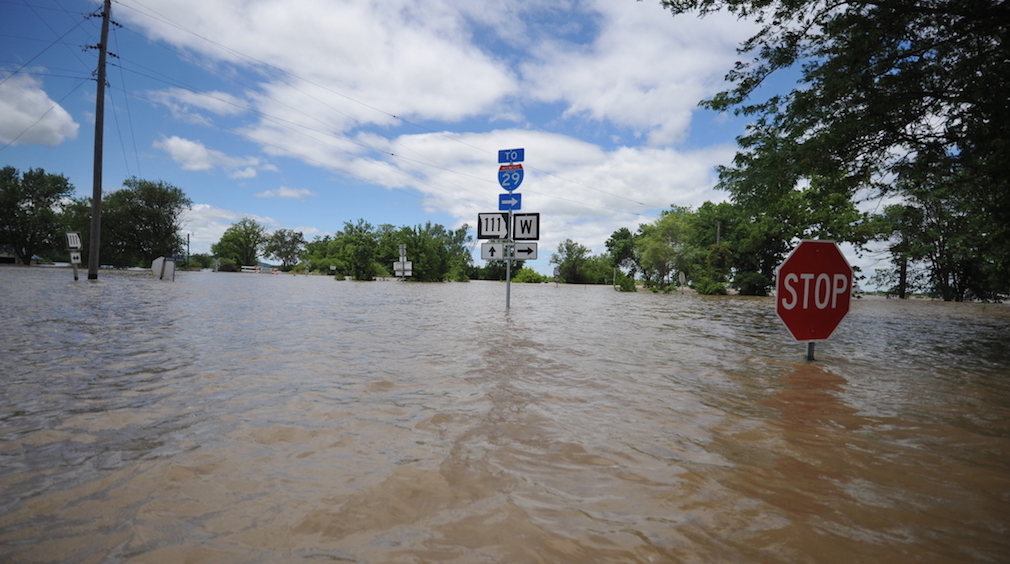
\includegraphics[width = 2.5in]{images/test_image15.jpg}} &
\subfloat[Hough Map]{\label{main:c}\includegraphics[width = 1.2in]{images/flood_easy5_hough.eps}}\\
\subfloat[Segmentation]{\label{main:d}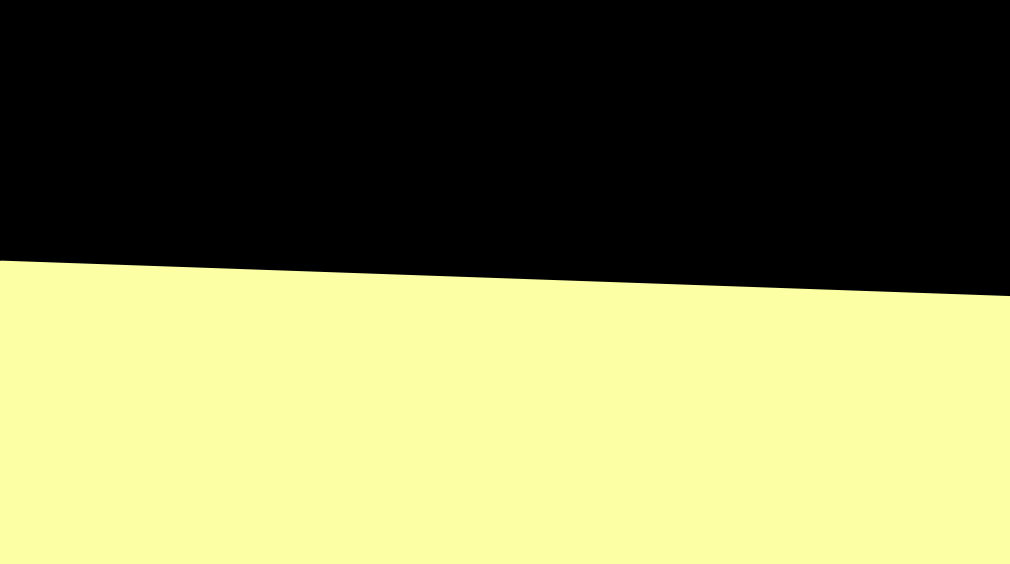
\includegraphics[width = 2.5in]{images/hough_image15.png}} &
\subfloat[Drawn Segmentation]{\label{main:d}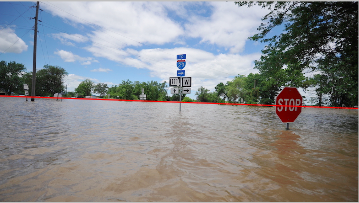
\includegraphics[width = 2.5in]{images/hough_drawn_image15.png}} 
\end{tabular}
\caption{Example of edge detection with Hough transformation for linear water horizon line.}
\label{fig:hough}
\end{figure}
In Figure \ref{fig:hough}, we apply edge detection with Hough transformation for a flood image with a slanted water horizon. We first take the input image, grayscale it, and determine the Canny edges contained in the image. We perform a Hough transformation to extract the edge features of the image and select the curve with the highest peak. As the figure illustrate, we were able to accurately find the horizon line even with a slanted water horizon and the presence of two objects. 

Note that edged-based HLD is very elementary and not applicable for most images as it assumes the horizon line is linear. As it is simply a horizontal partitioning of an image, HLD will not work very well for images with non-linear horizon. In addition, the flood water horizon might not be the most prominent line (i.e., the maximum peak might not correspond to the flood water horizon) which will cause the algorithm to incorrectly segment.

\subsubsection{Algorithm 2: Flood Segmentation via SLIC}

Current state-of-the-art algorithms in image processing uses \emph{superpixels}, an image patch better aligned with intensity edges than rectangular pixel grids. A very efficient and popular segmentation algorithm of superpixels called \emph{Simple Linear Iterative Clustering} (SLIC) was presented in \cite{achanta}. Given the number of clusters and weighing between pixel space and intensity, SLIC uses the popular $k$-means to segment an image in a given color space based on the color and space proximity of a superpixel. A version of SLIC  called SLICO where the weights between color and space are chosen adaptively was also presented in \cite{achanta}.
\begin{figure}[h!]
\centering
\begin{minipage}{.5\linewidth}
\centering
\subfloat[Input Image]{\label{main:a}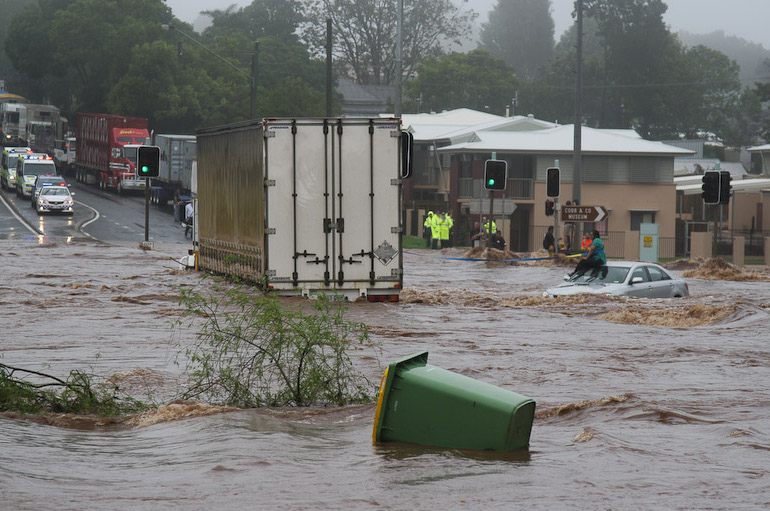
\includegraphics[scale=.20]{images/test_image22.jpg}}
\end{minipage}%
\begin{minipage}{.5\linewidth}
\centering
\subfloat[Segmentation]{\label{main:b}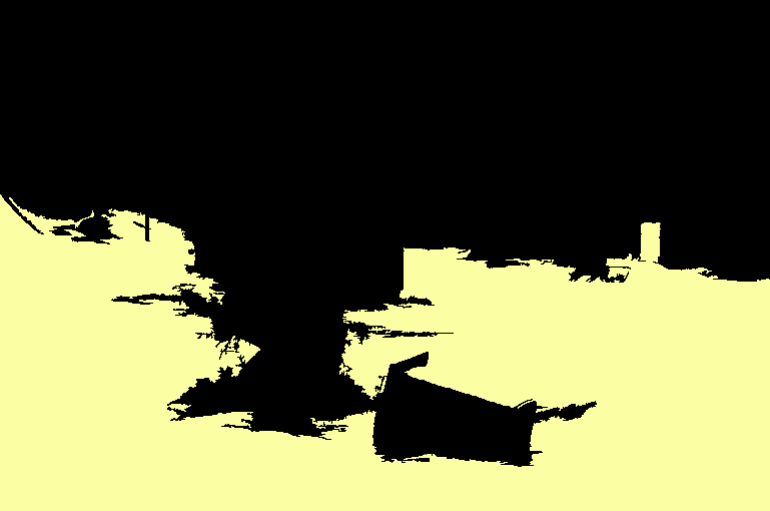
\includegraphics[scale=1.5]{images/SLIC_image22.png}}
\end{minipage}\par\medskip
\centering
\subfloat[Drawn Segmentation]{\label{main:c}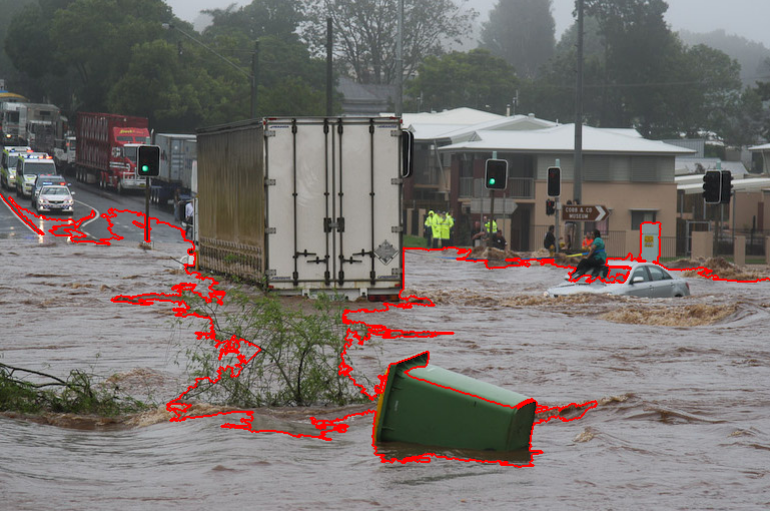
\includegraphics[scale=1.5]{images/SLIC_drawn_image22.png}}
\caption{SLIC using 2 clusters and compactness of 0.1.}
\label{fig:slic}
\end{figure}

We implement SLIC with $k=2$ in Figure \ref{fig:slic} for an image containing a nonlinear water horizon and different objects in the water. Although not perfectly accurate, we see that the algorithm was able to reasonably segment the flood region and non-flood region as two clusters. SLIC works reasonably well for images with multiple or ambiguous flood water horizon and images with a large number of objects. It is also efficient and scalable for large image or a collection of images.

\subsection{Deep Learning for Flood Images}

The current state-of-the-art algorithms for segmentation in computer vision uses \emph{deep learning} in the form of \emph{convolutional neural networks} (CNNs) \cite{schmidhuber, long, girshick}. Unlike the traditional machine learning approach which requires manual feature extraction before application of learning, CNNs employs \emph{end-to-end learning} where features are trained jointly with the classification task.

CNNs enable us to extend the image segmentation to \emph{semantic segmentation}. Recall that our image segmentation problem involves partition of an image into a flood region and a non-flood region. The two algorithms we had presented performs this segmentation but the resulting image contains no information on what these segmented parts actually represents. That is, we know which part consists of flood water through manual inspection only. Semantic segmentation involves the partition of an image into semantically meaningful parts with class labels on each parts.

Training a CNNs for semantic segmentation requires a large amount of data and computational power. However, training from scratch is often not necessary as one can employ \emph{transfer learning} (also referred to as \emph{fine-tuning}), improving a learner from one domain by transferring information from a related domain \cite{weiss}. We will present a pre-trained CNN model called \emph{fully convolutional neural networks} (FCN) that is applicable to our problem proposed in the works of \cite{long}. Here, ``fully" indicates that the neural network is composed of convolutional layers are without any fully-connected layers or multilayer perception usually found at the end of the network.

\subsubsection{Algorithm 3: Flood Segmentation via FCN}

We use the weights of the FCN model trained on the PASCAL-Context dataset which consists of over 400 labels for 10,103 images \cite{mottaghi}. The network consists of 18 convolution layers, 5 pooling layers and 15 rectified linear units to apply the activation function $f(x) = max(0,x)$ after each convolution. The output is a segmented image with scores associated with each of the 400 labels.

We take the score associated with the label ``water" and compute the mean of the label score for each region. Each pixel with a water score greater than or equal to the mean of the label is classified as a flood pixel. Note, while we can define any percentile of scores to classify, we found that the mean score works best as anything higher results in a high number of false positives and anything lower results in a high number of false negatives.

\section{Evaluation}

\subsection{Metrics}By far the best algorithm is FCN which has a mean pixel accuracy of 91\% and a mean IU score of 84\%.

The output of each algorithm is compared to the labeled image using two metrics: (1) pixel accuracy and (2) mean intersection over union (IU) score (also known as the Jaccard index). Pixel accuracy is simply the number of pixels correctly labeled divided the total number of pixels in the image. The IU score is the number of true positives divided by the sum of true positives, false positives and false negatives over each class. The latter metric is often the standard in the computer vision literature.

More formally, define $n_{ij}$ be the pixel of class $i$ predicted to belong to class $j$ and $t_i = \sum_j n_{ij}$ be the total number of pixels of class $i$. The metrics are given as follows:
\begin{enumerate}
\item Pixel Accuracy = $\frac{\sum_n n_{ii}}{\sum_i t_i}$
\item Mean IU Score = $ \frac{1}{n_{cl}} \sum_i \frac{n_{ii}}{t_i + \sum_j n_{ji} - n_{ii}}$
\end{enumerate}

\subsection{Result}

The mean pixel accuracy and IU score over the entire crowdsource flood image dataset is given in Table \ref{tab:result}. We see that simply using Hough transformation for image partitioning correctly classified approximately 80\% of the pixels which is slightly better than SLIC. However, in considering the mean IU score where there is a greater penalty for misclassification, SLIC performs better than Hough. 
\begin{table}[h!]
\centering
\caption{Comparison of result on flood image dataset.}
\label{tab:result}
\begin{tabular}{l|ll}
{\bf Algorithm} & {\bf Mean Pixel Accuracy} & {\bf Mean IU Score} \\
\hline
{\bf Hough}     & 0.7968         & 0.6696   \\
{\bf SLIC}      & 0.7828         & 0.6899   \\
{\bf FCN}      & 0.9125         & 0.8415  
\end{tabular}
\end{table}
While the overall results suggests that Hough and SLIC are comparable, if we examine specific cases, the difference between the two are very pronounced. Consider the example is given in Figure \ref{fig:result_example1} where we see that SLIC gives a much better segmentation when the most prominent line does not correspond to the flood water horizon. 

\begin{figure}[h!]
\centering
\begin{tabular}{ccc}
\subfloat[Input Image]{\label{main:a}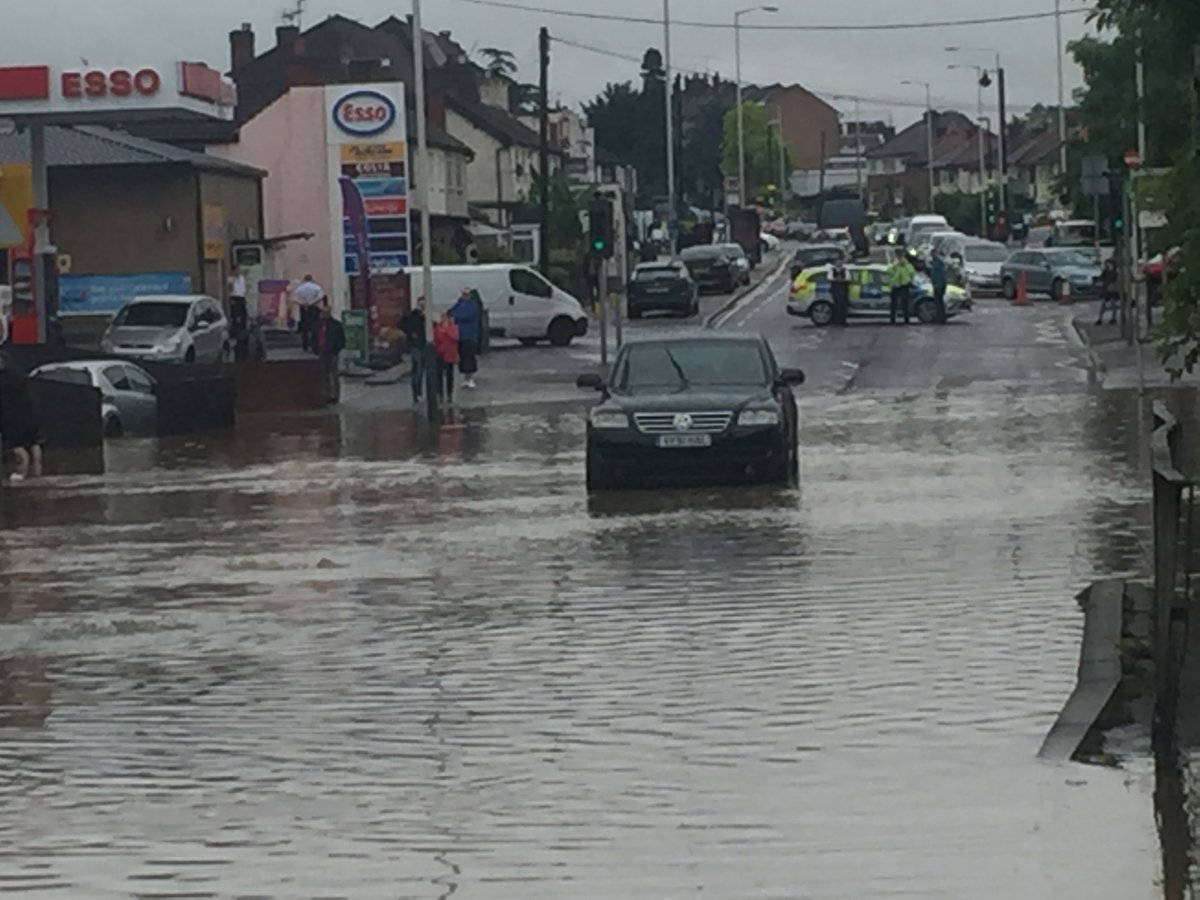
\includegraphics[width = 1.8in]{images/test_image10.jpg}} &
\subfloat[Truth (Acc. = 1, IU = 1)]{\label{main:c}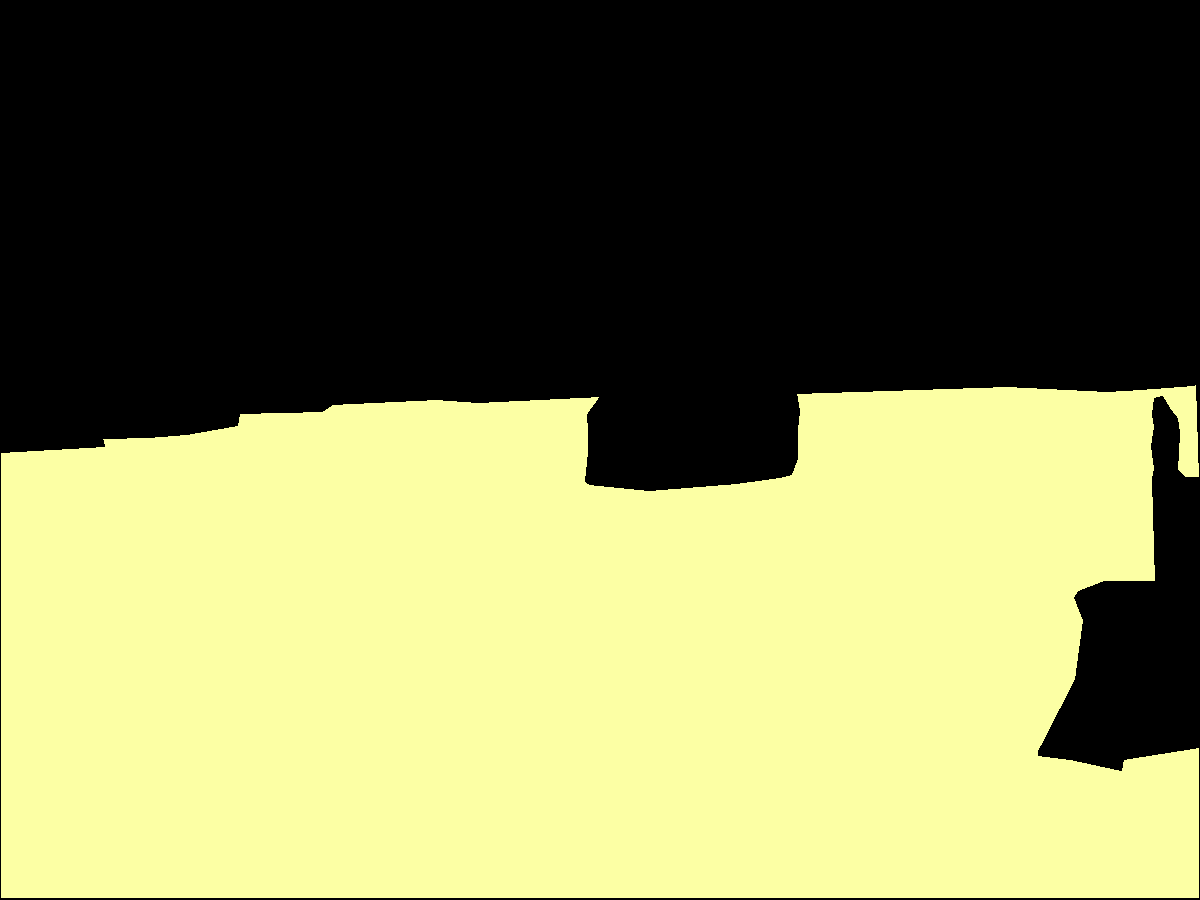
\includegraphics[width = 1.8in]{images/truth_image10.png}} &
\subfloat[Hough (Acc. = 0.60, IU = 0.37)]{\label{main:c}
\includegraphics[width = 1.8in]{images/hough_image10.png}} \\
\subfloat[SLIC (Acc. = 0.89, IU = 0.80)]{\label{main:d}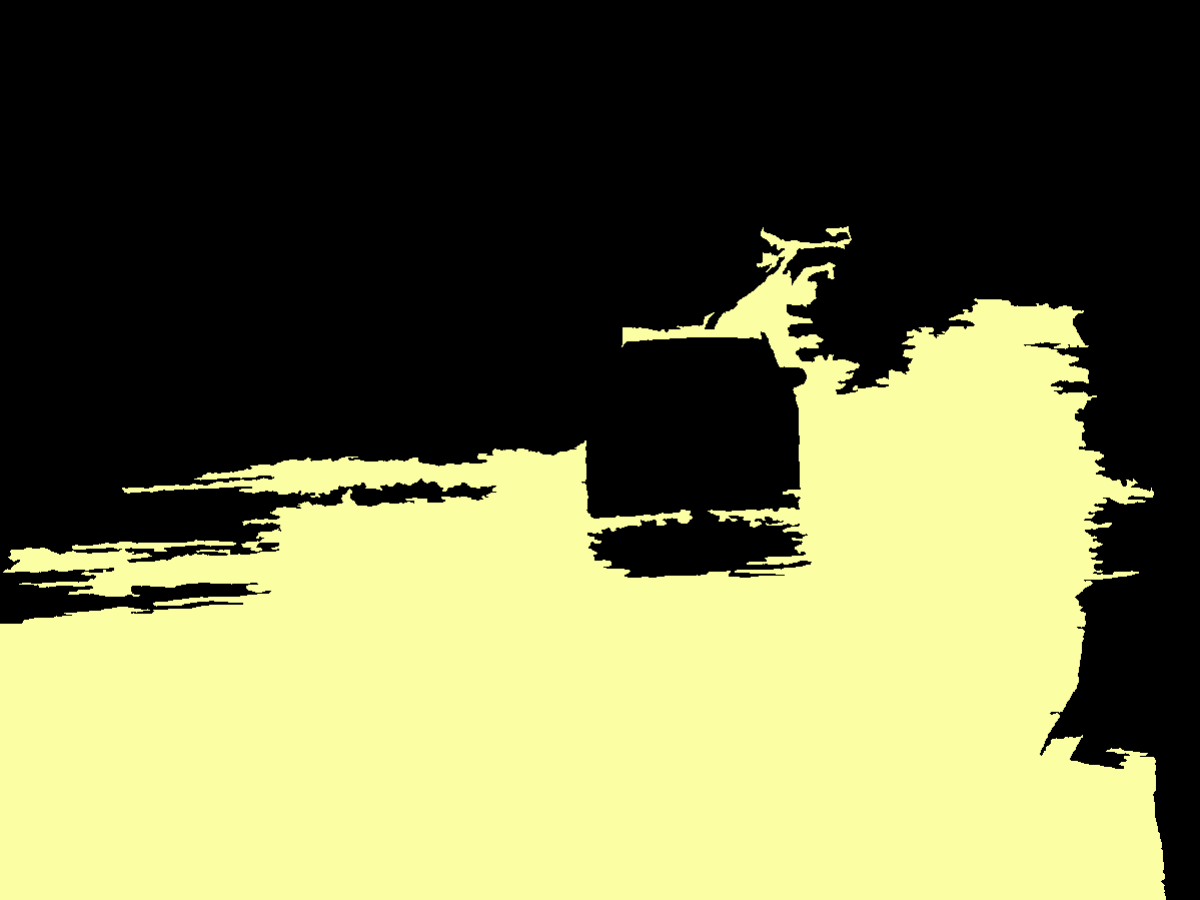
\includegraphics[width = 1.8in]{images/SLIC_image10.png}} &
\subfloat[FCN (Acc. = 0.93, IU = 0.86)]{\label{main:e}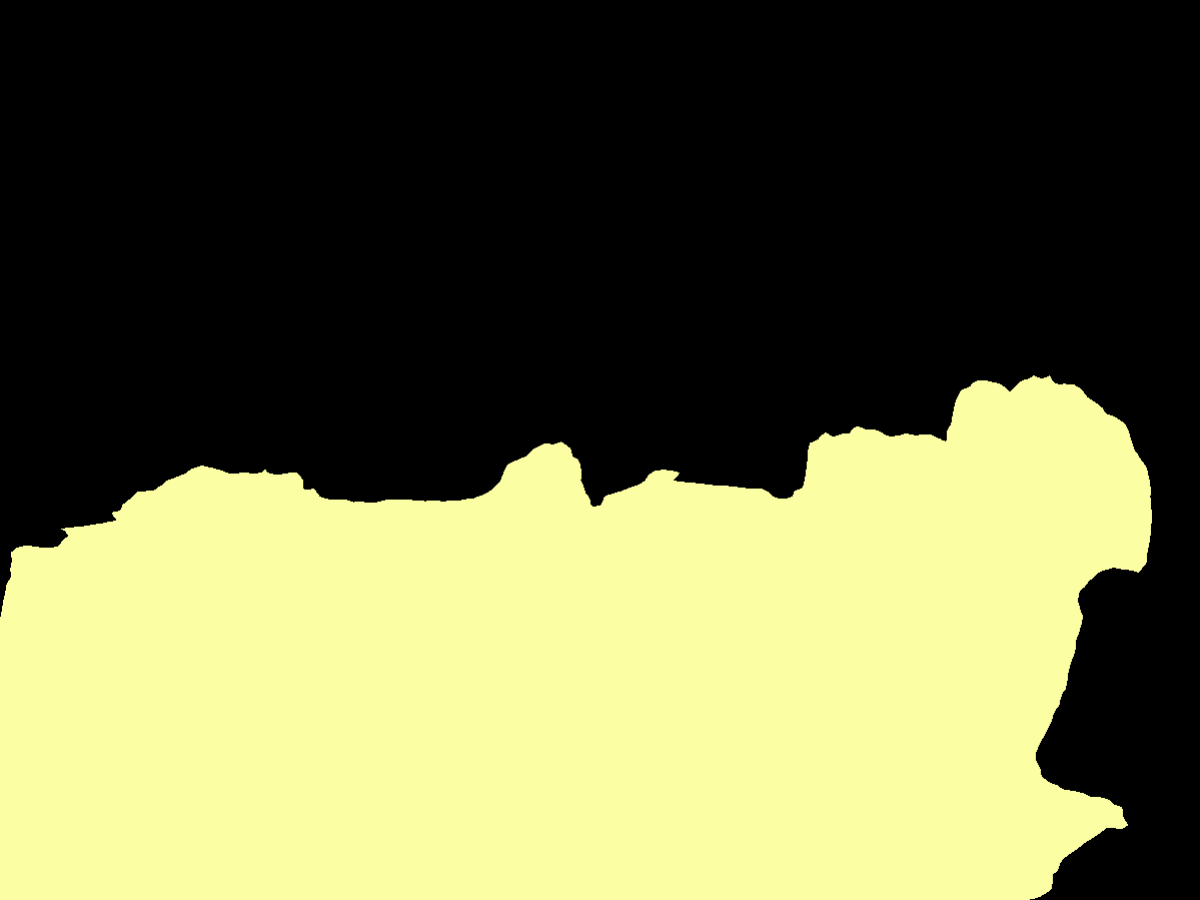
\includegraphics[width = 1.8in]{images/FCN8_image10.png}} 
\end{tabular}
\caption{Example result of each algorithm for a test image.}
\label{fig:result_example1}
\end{figure}

Although the pixel accuracy for both Hough and SLIC are very high, the overall IU score suggests that they are not that reliable. By far the best algorithm is FCN which has a mean pixel accuracy of 91\% and a mean IU score of 84\%. The major advantage of FCN is that it is able to segment objects contained in the flood better than SLIC. We show an example of such case in Figure \ref{fig:result_example2} where FCN was able to segment the raft, dog and human from the flood water.

\begin{figure}[h!]
\centering
\begin{tabular}{ccc}
\subfloat[Input Image]{\label{main:a}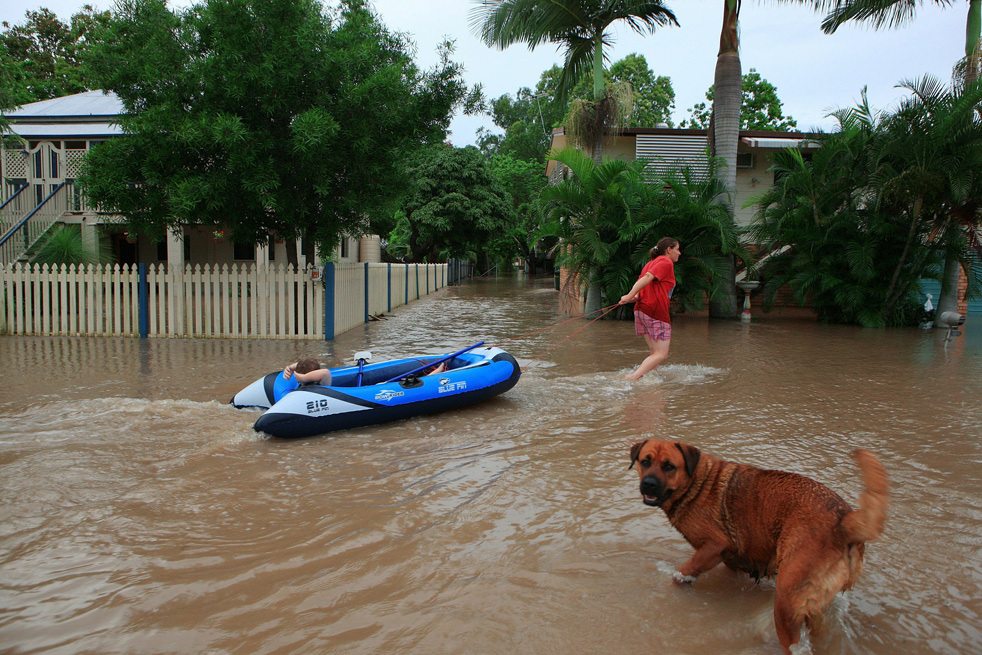
\includegraphics[width = 1.8in]{images/test_image9.jpg}} &
\subfloat[Truth (Acc. = 1, IU = 1)]{\label{main:b}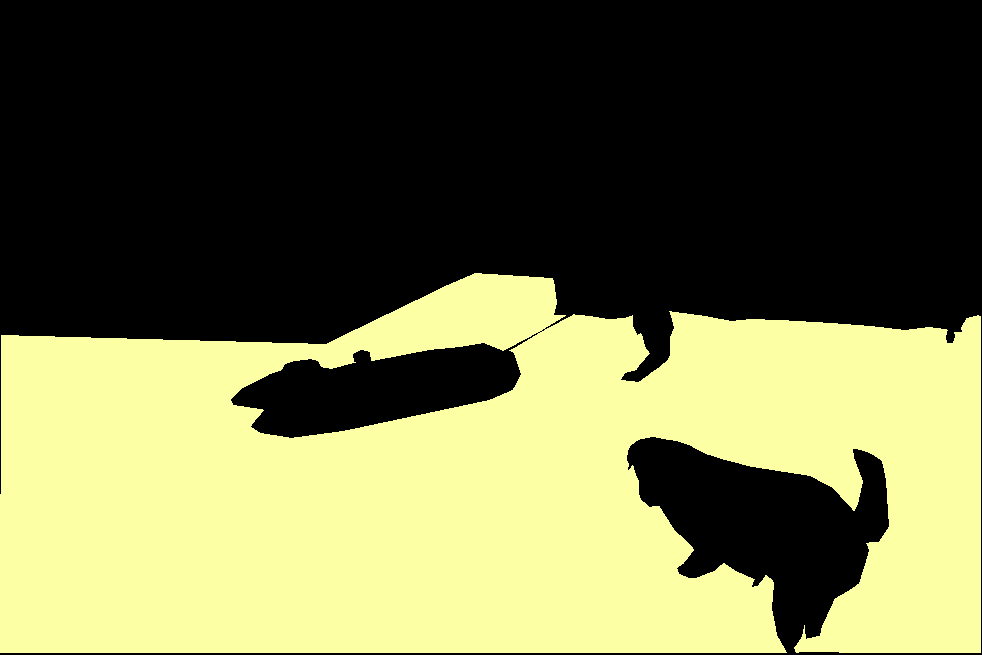
\includegraphics[width = 1.8in]{images/truth_image9.png}} &
\subfloat[Hough (Acc. = 0.83, IU = 0.71)]{\label{main:c}
\includegraphics[width = 1.8in]{images/hough_image9.png}}  \\
\subfloat[SLIC (Acc. = 0.84, IU = 0.72)]{\label{main:d}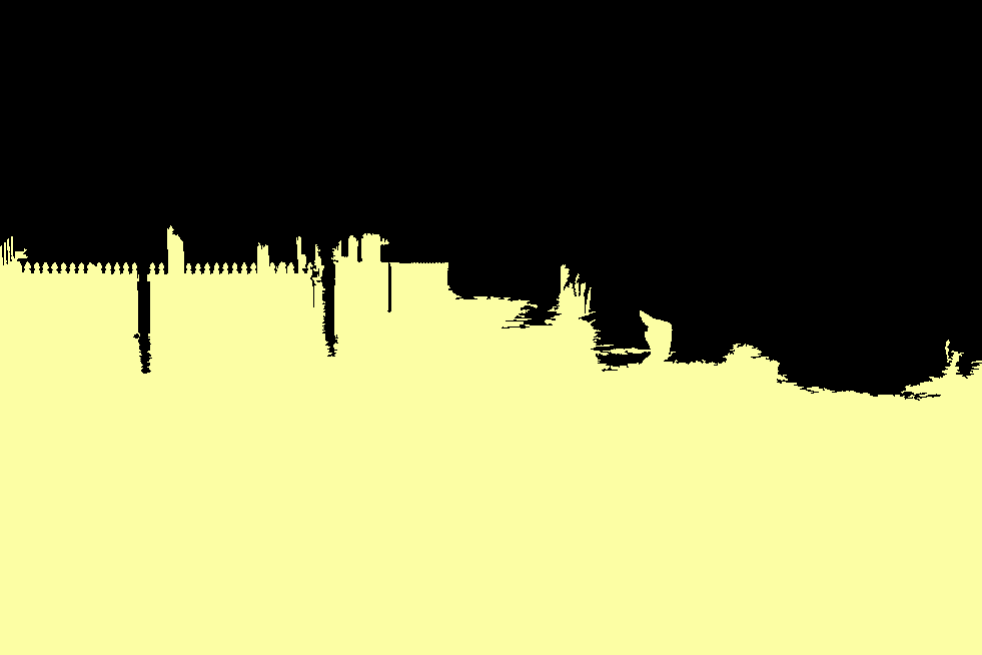
\includegraphics[width = 1.8in]{images/SLIC_image9.png}} &
\subfloat[FCN (Acc. = 0.94, IU = 0.88)]{\label{main:e}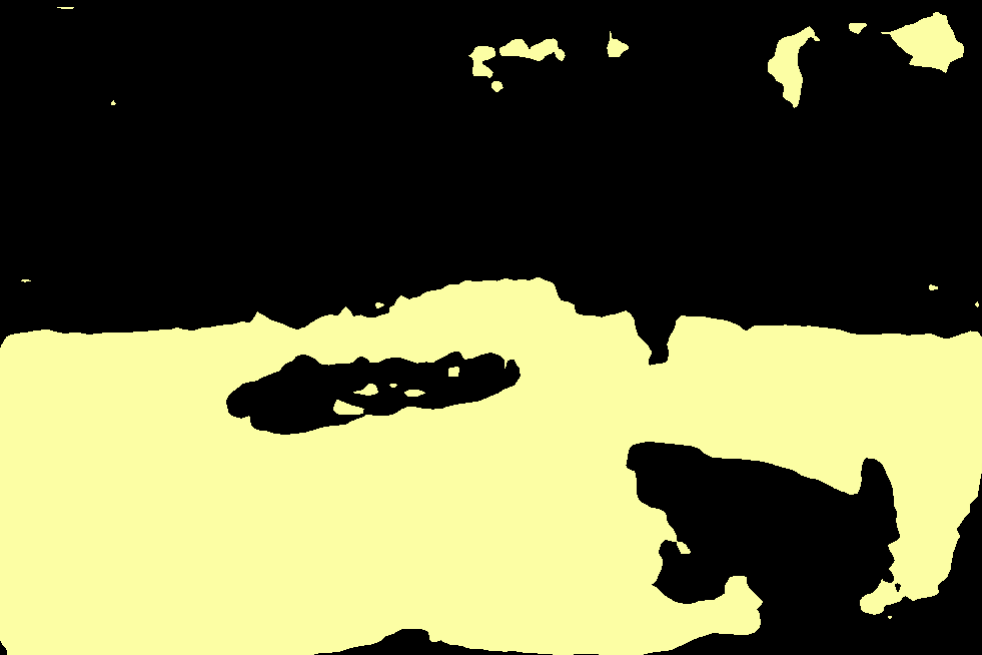
\includegraphics[width = 1.8in]{images/FCN8_image9.png}} 
\end{tabular}
\caption{Example result of each algorithm for a test image.}
\label{fig:result_example2}
\end{figure}


\subsection{Drawbacks of Hough and SLIC}

Hough transformation works very well for flood images where the horizon line is linear and prominent. If there are other prominent lines contained in the picture, there will multiple peaks in the Hough map and the water horizon is not guaranteed to correspond to the highest peak. In Figure \ref{fig:hough_fail}, the most prominent line corresponds to the roof of a building so the water horizon was not captured. While there are some advanced edge detection techniques which can handle non-linear horizons, most image processing techniques lacks the ability to segment objects from flood water.
\begin{figure}[h!]
\centering
\includegraphics[scale=0.4]{images/hough_incorrect.eps}
\caption{Hough transformation fails to capture the water horizon.}
\label{fig:hough_fail}
\end{figure}

The main problem with unsupervised methods like SLIC is that it is not clear how we set the number of clusters. We can have vastly different segments or even no segments at all depending on the value of $k$. Another problem is the presence of specularity (i.e., reflections) in an image. SLIC tends to cluster pixels found in reflective regions of the image.
\begin{figure}[h!]
\begin{minipage}{.3\linewidth}
\centering
\subfloat[SLIC with $k=3$]{\label{main:a}\includegraphics[width = 2.5in]{images/kmeans4_seg3.eps}}
\end{minipage}
\begin{minipage}{.8\linewidth}
\centering
\subfloat[SLIC with $k=4$]{\label{main:b}\includegraphics[width = 2.5in]{images/kmeans4_seg4.eps}}
\end{minipage}\par
\begin{minipage}{.3\linewidth}
\centering
\subfloat[SLIC with $k=3$]{\label{main:a}\includegraphics[width = 2.5in]{images/kmeans5_seg3.eps}}
\end{minipage}
\begin{minipage}{.8\linewidth}
\centering
\subfloat[SLIC with $k=4$]{\label{main:b}\includegraphics[width = 2.5in]{images/kmeans5_seg4.eps}}
\end{minipage}\par
\caption{SLIC segments is highly dependent on the defined number of clusters and the presence of specularity.}
\label{fig:slico_wrong}
\end{figure}

In Figure \ref{fig:slico_wrong}(a), we see that $k=3$ provides a reasonable segmentation for the image. However, when we set $k=4$ in Figure \ref{fig:slico_wrong}(b), the segmentation changes greatly to something highly inaccurate. For a different input image shown in Figure \ref{fig:slico_wrong}(c), $k=3$ does even not provide any segments as every pixel is grouped into the same cluster. When we increase $k=4$ in Figure \ref{fig:slico_wrong}(d), we see that specularity region in the flood water becomes a cluster. While it is possible to improve segmentation accuracy through specularity removal, such task is non-trivial.

If we assume the image contains no specularity, then SLICO with $k$ between 2 to 3 will give fairly good results. However, our goal is to be able to perform segmentation without such assumption. In addition, we would like a parameter-free model which would work for all flood images.


\section{Conclusion}\label{sec:conclusion}

This study present several different approaches for flood water segmentation for crowdsourced images. We found that using a pre-trained convolutional neural networks, we showed that it is possible to perform parameter-free flood water segmentation using just a single image without any stringent assumptions on image content. The model's accuracy is limited due to the lack of a labeled database of flood images. A natural extension is to perform fine tuning or transfer learning of the model on a large, labeled flood image dataset. It would also be of interest to examine all the contents of an image and see if we can use such information for flood damage assessment and flood monitoring.

\section*{References}

\bibliographystyle{plain}
\bibliography{floods_bib}

\end{document}